\documentclass{beamer}

\usepackage[portuguese]{babel}
\usepackage[utf8]{inputenc}
\usepackage{minted}

\title{Introdução}
\author[João Marcelo Uchôa de Alencar]{João Marcelo Uchôa de Alencar}
\institute{Universidade Federal do Ceará - Quixadá}

\begin{document}
   \begin{frame}
      \titlepage
   \end{frame}


\begin{frame}
   \frametitle{Apresentação}
   \begin{itemize}
      \item Professor João Marcelo Uchôa de Alencar.
      \item E-mail para contato: joao.marcelo@ufc.br.
      \item Programa da disciplina: \url{http://www.joao.marcelo.nom.br/}.
      \item Avaliações:
      \begin{itemize}
         \item 4 avaliações 
	      \begin{itemize}
            \item 3 Notas das atividades, das quais pegamos as \textbf{2 maiores}.
            \item 1 Nota do Seminário.
         \end{itemize}
	      \item Fazer a média dessas 3 notas. 
      \end{itemize}
      \item Proposta: não ter prova final, aqueles que tiveram acima de 5,0 estão aprovados. Caso contrário, reprovados.
   \end{itemize}
\end{frame}


\begin{frame}
   \frametitle{História dos Sistemas UNIX}
   \begin{itemize}
      \item Unix foi desenvolvido pelo \textit{Bell Labs} logo após esse laboratório abandonar o projeto \textit{Multics}.
      \item Algumas decisões de projeto foram reaproveitadas do \textit{Multics}
      \begin{itemize}
         \item Dispositivos como arquivos.
	 \item Interpretador de comandos como processo independente do \textit{kernel}.
      \end{itemize}
      \item O \textit{Bourne Shell} e a linguagem \textit{awk} foram incluídos na versão 7 do UNIX.
      \item Um foco forte na criação de ferramentas para processamento textual.
      \item Padrão POSIX.
   \end{itemize}
\end{frame}

\begin{frame}
   \frametitle{História dos Sistemas UNIX}
   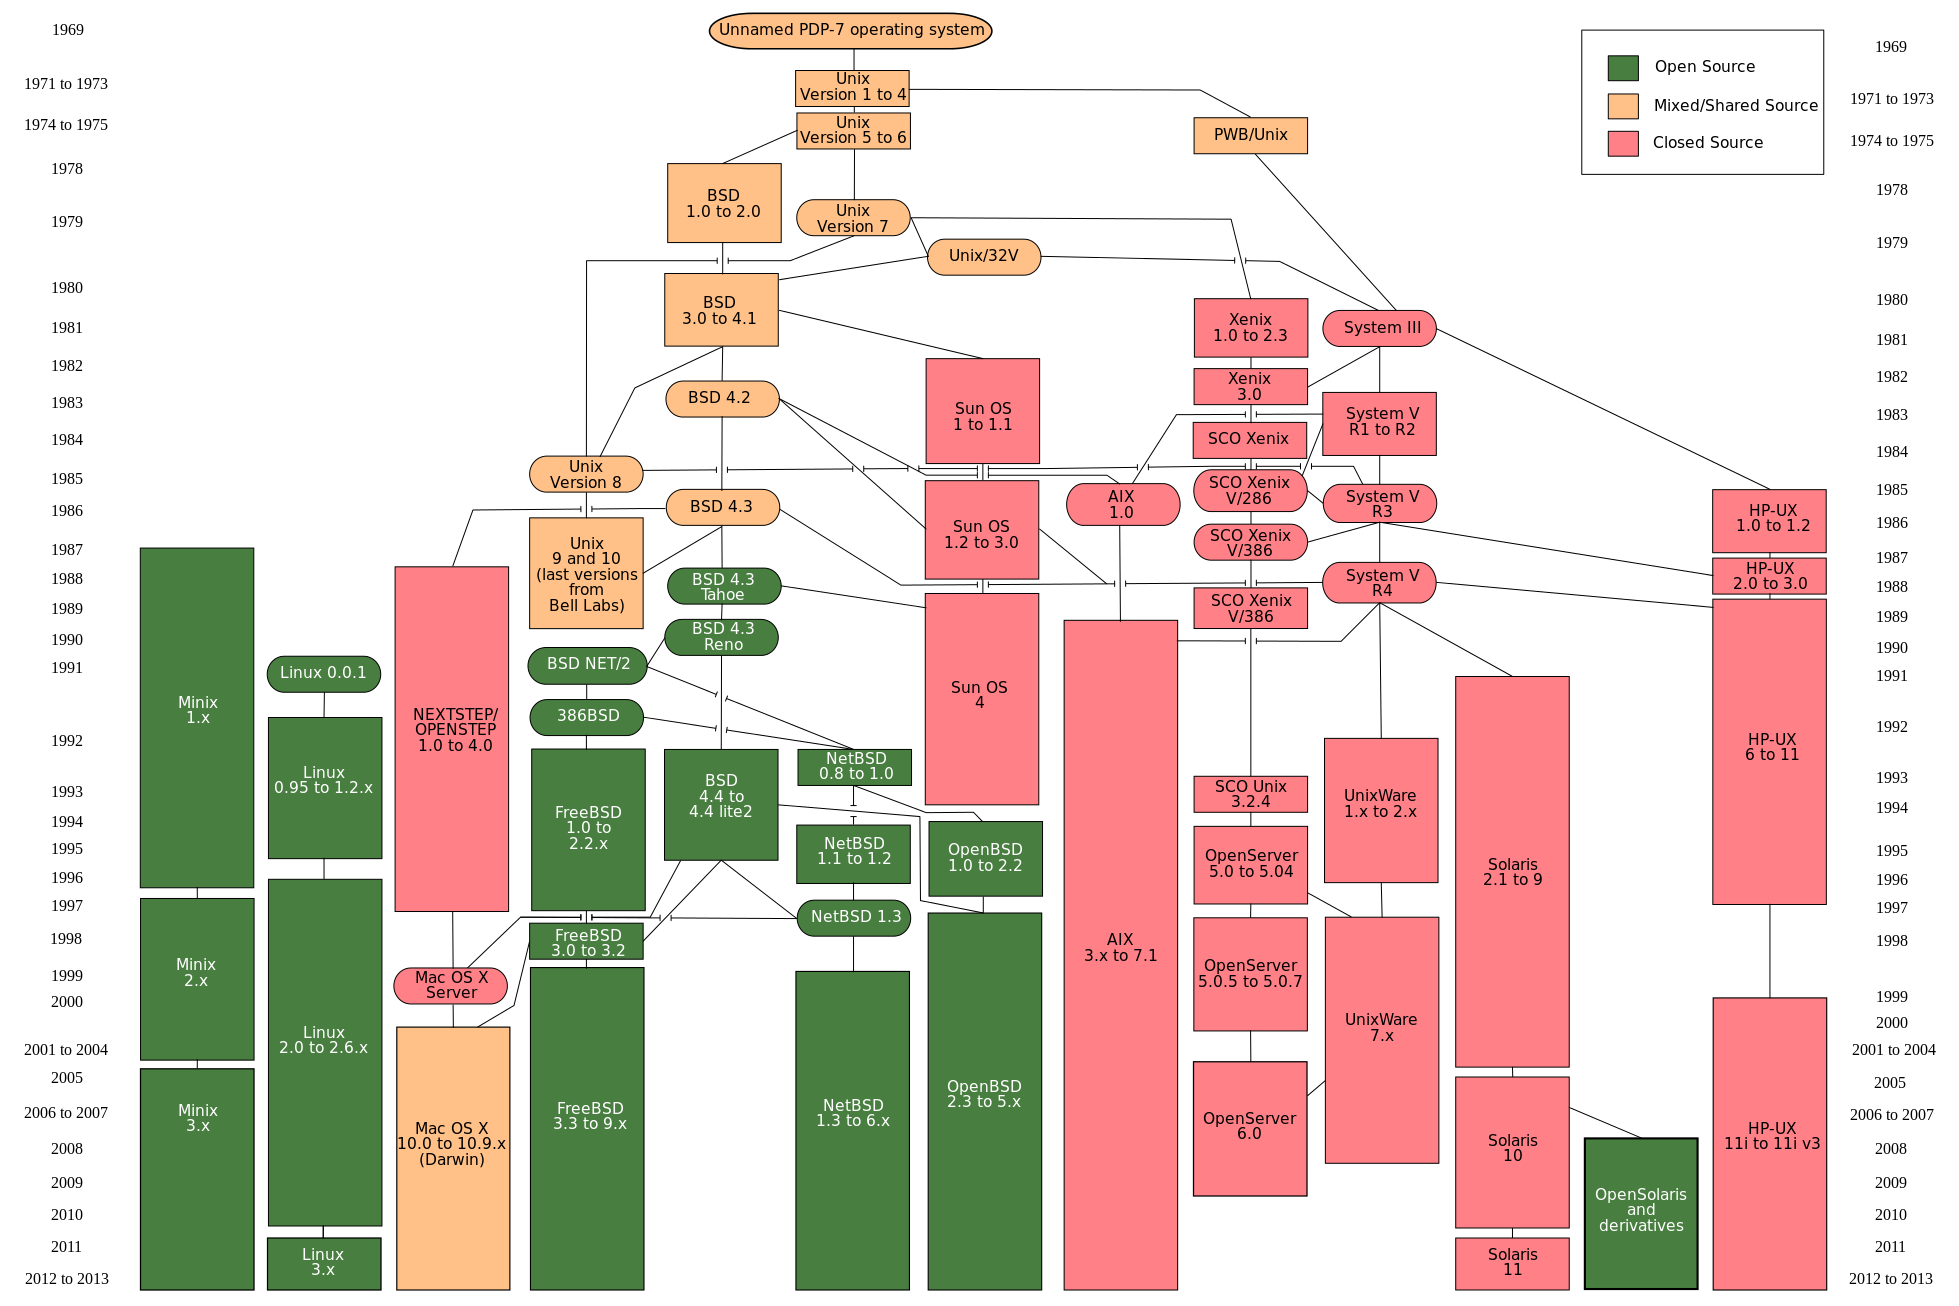
\includegraphics[scale=0.17]{figuras/Unix_history-simple.png}
\end{frame}

\begin{frame}
   \frametitle{Princípios Para Ferramentas de \textit{Software}}
   Os ambientes UNIX obedecem os seguintes princípios no desenvolvimento de suas ferramentas:
   \begin{itemize}
      \item Cada ferramenta deve oferecer apenas uma \textbf{funcionalidade} e implementá-la da melhor maneira.
      \item Processar \textbf{linhas de texto}, evitar dados binários.
      \item Aproveitar o poder das \textbf{expressões regulares}.
      \item Utilizar a \textbf{saída padrão} para troca de dados.
      \item Evitar \textbf{mensagens desnecessárias} no terminal.
      \item Utilizar para a saída o \textbf{mesmo formato} da entrada.
      \item Reutilizar programas \textbf{existentes}.
      \item Tente \textbf{generalizar} suas ferramentas.
   \end{itemize}
\end{frame}

\begin{frame}
   \frametitle{Linguagens de \textit{Scripting} versus Linguagens Compiladas}
   \begin{itemize}
      \item Programas escritos em linguagens compiladas são traduzidas do seu \textbf{código fonte} original para o \textbf{código objeto} da máquina alvo.
      \item A vantagem é que são programas eficientes, a desvantagem é que atuam em baixo nível.
      \item Exemplo da desvantagem: escrever em C um programa que copie todos arquivos de um diretório para outro.
      \item Linguagens de \textit{script} são interpretadas, um \textbf{interpretador} ler cada linha do \textit{script} e usa funções internas para executá-las.
   \end{itemize}
\end{frame}

\begin{frame}
   \frametitle{O que é o \textit{Shell}?}
   \centering
   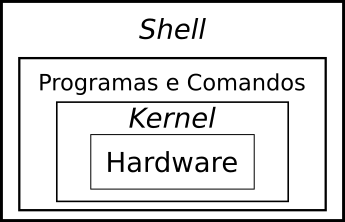
\includegraphics[scale=0.8]{figuras/camadas.png}
\end{frame}

\begin{frame}[fragile]
      \frametitle{O que é o \textit{Shell}?}
	      \scriptsize
      \begin{block}{Ao nível do \textit{Shell}:}
      \begin{minted}{bash}
$ ls 
'Área de trabalho'  Documentos  Downloads  Dropbox  Imagens  Modelos  Música 
Público  Vídeos
      \end{minted}
      \end{block}
      \begin{block}{Ao nível do \textit{Kernel}:}
      \scriptsize
      \begin{minted}{bash}
execve("/usr/bin/ls", ["ls"], [/* 49 vars */]) = 0 
brk(NULL) = 0x5585c31e8000 
mmap(NULL, 4096, PROT_READ|PROT_WRITE, MAP_PRIVATE|MAP_ANONYMOUS, -1, 0) 
access("/etc/ld.so.preload", R\_OK) = -1 ENOENT (No such file or directory) 
open("/etc/ld.so.cache", O\_RDONLY|O\_CLOEXEC) = 3 
fstat(3, {st\_mode=S\_IFREG|0644, st\_size=101277, ...}) = 0 
...
      \end{minted}
      \end{block}
\end{frame}

\begin{frame}
   \frametitle{O que é \textit{Shell}?}
   \begin{center}
   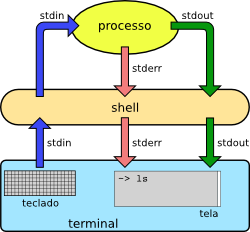
\includegraphics[scale=1.0]{figuras/funcionamento_terminal.png}
   \end{center}
   \tiny
   Fonte: \url{http://wiki.inf.ufpr.br/maziero/doku.php?id=unix:shell_avancado}
\end{frame}

   \begin{frame}
      \frametitle{O que é o \textit{Shell}?}
      \begin{itemize}
         \item O \textit{shell} é simplesmente o programa que lê o comando que você teclou e o converte em uma forma mais simplificada e legível ao sistema operacional (\textit{kernel}). 
         \item Também fornece uma \textbf{linguagem} para organizar uma sequência de comandos em um scripts, permitindo a automização de tarefas administrativas. 
	 \item Um dos grandes diferencias é permitir invocar programas feitos em outras linguagens sem dificuldade.
	 \item A troca de dados entre programas é feita em formato de linhas de \textbf{texto simples}.
      \end{itemize}
   \end{frame}

   \begin{frame}
      \frametitle{Tarefas do \textit{Shell}}
      \begin{itemize}
         \item Exame da linha de comandos recebida.
         \item Atribuição e substituição de sariáveis.
         \item Resolução de redirecionamentos.
         \item Substituição de metacaracteres.
         \item Criação de processos filhos para executar comandos.
      \end{itemize}
   \end{frame}

   \begin{frame}
      \frametitle{Principais versões do \textit{Shell}}
      \begin{itemize}
         \item Bourne Shell (sh)
         \item Bourne Again Shell (bash)
         \item Korn Shell (ksh)
         \item C Shell (csh)
      \end{itemize}
   \end{frame}

\begin{frame}
   \frametitle{Por que usar \textit{Shell}?}
   \begin{itemize}
      \item É mais fácil lidar com arquivos e diretórios em \textit{Shell}, assim iniciar ou finalizar outros programas.
      \item O desempenho costuma ser pior, mas o tempo de programação é bem menor do que em linguagens compiladas.
      \item Simplicidade.
      \item Portabilidade.
      \item Facilidade de desenvolvimento.
   \end{itemize}
\end{frame}


\begin{frame}[fragile]
   \frametitle{Um primeiro exemplo - Contando os Usuários}
   \begin{minted}{bash}
   $ who
   $ who | wc -l
   $ cat > usuarios.sh
   who | wc -l
   ^D
   $ chmod +x usuarios.sh
   $ ./usuarios
   \end{minted}
\end{frame}

\begin{frame}[fragile]
   \frametitle{Um primeiro exemplo - Contando os Usuários}
   \begin{itemize}
      \item Qualquer sequência de comandos, dentro de um arquivo de texto, com permissão para execução, vira um \textit{shell script}.
      \item Ao perceber que não é um arquivo compilado, o \textit{kernel} retorna o arquivo ao \textit{shell}, que o executa com o \textit{shell} padrão do sistemas.
      \item Mas como existem vários \textit{shells}, é boa prática especificar qual você deseja utilizar. 
   \end{itemize}
\end{frame}

\begin{frame}[fragile]
   \frametitle{Um primeiro exemplo - Contando os Usuários}
   \begin{minted}{bash}
   $ cat usuarios.sh 
   #!/bin/bash
   who | wc -l 
   \end{minted}
   Neste contexto, o seguinte comando: 
   \begin{minted}{bash}
   $ ./usuarios.sh
   \end{minted}
   equivale a:
   \begin{minted}{bash}
   $ /bin/bash usuarios.sh
   \end{minted}
\end{frame}

\begin{frame}
   \frametitle{OFF-TOPIC: Como Usar o SSH/SCP}
   \begin{itemize}
      \item O SSH é um protocolo para \textit{login} remoto que utiliza criptografia para proteger a troca de informações.
      \item O comando \textit{ssh} no Linux implementa o lado cliente do protocolo.	
      \item O protocolo SSH também pode ser usado para transferir arquivos, não só enviar comandos.
      \item O comando \textit{scp} permite a cópia de arquivo entre cliente e servidor e também entre dois servidores remotos.
      \item A vantagem é que toda a comunicação é criptografada e protegida por senha.
   \end{itemize}
\end{frame}

\begin{frame}[fragile]
   \frametitle{Acessando um Servidor com SSH}
   Se você simplesmente fizer isso:
   \begin{minted}{bash}
   $ ssh 200.19.176.156
   \end{minted}
   ou
   \begin{minted}{bash}
   $ ssh programacaoscripts.joao.marcelo.nom.br
   \end{minted}
   \begin{itemize}
      \item O cliente \textit{ssh} vai tentar logar no servidor remoto (200.19.176.156 ou programacaoscripts.joao.marcelo.nom.br) usando o usuário que você está logado no sistema local.
      \item \textbf{Exemplo:} se seu usuário local for \textit{alunoufc}, o cliente irá tentar logar como \textit{alunoufc} na máquina remota.
   \end{itemize}

   Caso o usuário local não exista no servidor e deseje utilizar outro:
   \begin{minted}{bash}
$ ssh joaomarcelo@programacaoscripts.joao.marcelo.nom.br
   \end{minted}
\end{frame}

\begin{frame}[fragile]
   \frametitle{Acessando um Servidor com SSH}
   Quando você acessa um servidor pela primeira vez:
   \small
   \begin{minted}{bash}
The authenticity of host '18.213.179.235' can't be established.
ECDSA key fingerprint is SHA256:LKdo00AkJT7haicaM.
Are you sure you want to continue connecting (yes/no)?    
   \end{minted}
   \normalsize
   \begin{itemize}
      \item É apenas uma confirmação, digitando \textit{yes} ela não aparece nas próximas conexões.
      \item Partimos para a parte de autenticação, que irá requisitar uma senha.
      \item Se a senha informada for correta, \textbf{sucesso}, você está logado no servidor.
   \end{itemize}
\end{frame}

\begin{frame}
   \frametitle{Autenticação no Servidor SSH}
   Utilizar senhas tem seus problemas:
   \begin{itemize}
      \item Uma senha complexa é fácil de esquecer.
      \item O usuários acabam escolhendo senhas fáceis, que podem ser descobertas e causar problemas de segurança.
      \item Uma solução melhor e amplamente utilizada nas nuvens é o uso de um arquivo de identificação chamado \textbf{chave}.
      \item Cada arquivo de chave está associado com um usuário no servidor.
      \item O usuário deve ter cuidado para proteger sua chave, qualquer que tiver acesso à ela poderiá acessar o servidor.
   \end{itemize}
   A solução mais segura é exigir que o usuário forneça uma \textbf{senha e a chave} toda vez que for logar. Mas deixamos para aprender isso mais adiante no curso.
\end{frame}

\begin{frame}[fragile]
   \frametitle{Utilizando a Chave no SSH}
   \scriptsize
   \begin{minted}{bash}
$ ssh -i joaomarcelo.pem joaomarcelo@programacaoscripts.joao.marcelo.nom.br   
   \end{minted}
   \normalsize
   \begin{itemize}
      \item A chave é o arquivo \textit{joaomarcelo.pem}.
      \item O usuário remoto é \textit{joaomarcelo}. O nome do arquivo da chave e do usuário não precisam ser os mesmos.
      \item O servidor remoto é \textit{programacaoscripts.joao.marcelo.nom.br}.
      \item O usuário \textit{joaomarcelo} deve existir no servidor remoto e estar configurado para permitir o acesso via chave.
   \end{itemize}
   No Slack do curso já enviei a chave privada de cada um. Podem tentar fazer o \textit{login} agora.
   \begin{block}{Lembrete}
   A chave tem que ter permissões de acesso apenas para o usuário local. Portanto, confirme:
   \begin{minted}{bash}
   $ chmod 0600 joaomarcelo.pem
   \end{minted}
   \end{block}
\end{frame}

\begin{frame}[fragile]
   \frametitle{Copiando Arquivos via SCP - Formato Geral}
   \small
   \begin{block}{Copiando arquivos para o servidor}
   \scriptsize
   \begin{minted}{bash}
scp -i <chave> <arquivolocal> <usuario>@<servidor>:<diretorioremoto>
   \end{minted}
   \end{block}
   \normalsize
   \begin{block}{Copiando arquivos do servidor}
   \scriptsize
   \begin{minted}{bash}
scp -i <chave> <usuario>@<servidor>:<arquivoremoto> <arquivolocal>
   \end{minted}
   \end{block}
   Para copiar diretórios, podemos usar a opção $-r$.
\end{frame}

\begin{frame}[fragile]
   \frametitle{Copiando Arquivos via SCP - Exemplos}
   \small
   \textbf{Observação:} os comandos abaixos podem ser digitados na mesma linha. Coloquei em várias linhas para caber no \textit{slide}. A \textbackslash (barra)  pode ser usada para dividir um comando em várias linhas.
   \normalsize
   \begin{block}{Copiando arquivos para o servidor}
   \scriptsize
   \begin{minted}{bash}
scp -i joaomarcelo.pem teste.txt \
joaomarcelo@programacaoscripts.joao.marcelo.nom.br:/home/joaomarcelo/
   \end{minted}
   \end{block}
   \normalsize
   \begin{block}{Copiando arquivos do servidor}
   \scriptsize
   \begin{minted}{bash}
scp -i joaomarcelo.pem \
joaomarcelo@programacaoscripts.joao.marcelo.nom.br:/home/joaomarcelo/teste.txt \
teste.txt
   \end{minted}
   \end{block}
\end{frame}

\begin{frame}
   \frametitle{Regras Gerais para Atividades}
   \begin{itemize}
      \item \textbf{SEMPRE} leia com atenção todas as instruções.
      \item Obedeça observações sobre nome de pastas e arquivos no exercício.
      \item Se o exercício diz para criar uma pasta \textit{atividade01}, crie a pasta com o mesmo nome. Não use \textit{Atividade01}, \textit{atividade1}, \textit{aTivIDADE01}, etc.
      \item Na dúvida, pergunte ao professor.
      \item Muitas vezes usarei \textit{scripts} para correção. Se os nomes estiverem diferentes, o \textit{script} pode considerar a questão errada.
   \end{itemize}
\end{frame}

%\begin{frame}
%   \frametitle{Atividade 01 - Atividade de como usar o SSH/SCP}
%   \begin{enumerate}
%      \item Faça \textit{login} no servidor programacaoscripts.joao.marcelo.nom.br.
%      \item Crie a pasta \textit{atividades}.
%      \item Dentro da pasta \textit{atividades}, crie o diretório \textit{atividade01}.
%      \item Coloque o \textit{script} \textit{usuarios.sh} no diretório.
%      \item Execute o \textit{script} no servidor.
%   \end{enumerate}
%   Para colocar o \textit{script} no servidor, você pode editá-lo localmente e copiá-lo em seguida ou já editá-lo no próprio servidor, usando o \textit{nano} ou o \textit{vim}.
%\end{frame}

\end{document}

